\documentclass[uplatex,dvipdfmx,a4paper,11pt]{jsarticle}

\usepackage{amsmath,amsthm,amssymb}
\usepackage[dvipdfmx]{graphicx}
\usepackage{bm}
%
\usepackage{multirow}
\usepackage{wrapfig}

\usepackage{geometry}
\geometry{left=25truemm, right=25truemm, top=25truemm, bottom=25truemm}

%
\abovecaptionskip=-1pt
%\belowcaptionskip=-1pt
%
\renewcommand{\baselinestretch}{1.} %全体の行間調整
\renewcommand{\figurename}{Fig.}
\renewcommand{\tablename}{Tab.}
%
\makeatletter 
\def\section{\@startsection {section}{1}{\z@}{1.5 ex plus 2ex minus -.2ex}{0.5 ex plus .2ex}{\large\bf}}
\def\subsection{\@startsection{subsection}{2}{\z@}{0.2\Cvs \@plus.5\Cdp \@minus.2\Cdp}{0.1\Cvs \@plus.3\Cdp}{\reset@font\normalsize\bfseries}}
\makeatother 
%

\renewcommand{\thefootnote}{\fnsymbol{footnote}}

\pagestyle{empty}

\graphicspath{{../../figures//}}

\begin{document}

%%%%%%
% はじめに
%%%%%%
\begin{center}
{\Large \textgt{ランダムな接続性を有するネットワークポリマーの緩和挙動}}
\end{center}

\begin{flushright}
東亞合成 ${}^\circ$佐々木裕
\end{flushright}

% \vspace{-3mm}
\section{はじめに}
ゴムの高い破壊靱性の起源を説明するために、ヒステリシスロスなどのエネルギー散逸によって亀裂の伝播が抑制されるAndrewsのモデルが提案されている~\cite{andrews}。
ゴム弾性体の古典的なモデルである「アフィンネットワークモデル」からの発展形として、節点の揺らぎに着目した「ファントムネットワークモデル(PNM)」が提案された。
Flory によればメルト状態と同一なストランドのゆらぎを有するランダムネットワークにおいて PNM のふるまいを示すとされている~\cite{flory}。
我々は、この結節点のゆらぎ由来の散逸が、粘弾性的なエネルギー散逸モデルとなりうるのではないかと考え、これまで検討を進めている。

以前に、規則構造ネットワークの接続性をランダムへと変えることでPNM を再現できることを報告した~\cite{sasaki}。
ここでは、ランダムな連結性を持つネットワークポリマーの緩和挙動について、MDシミュレーションにより検討した結果を報告する。

% \vspace{-1mm}
\section{結果}
\subsection{シミュレーションについて}
既報~\cite{sasaki}に従い、ランダムな接続性を有する 3, 4 および 6 分岐のネットワークを作成した。
ストランドとして、セグメント間にLJ相互作用を導入したKG鎖と相互作用を入れないファントム鎖を用いた。
その平衡状態および変形(一軸伸張およびずりせん断)時の振る舞いについて、 OCTA 上の COGNAC シミュレーターを用いた分子動力学シミュレーションにより評価した。

\subsection{力学応答の評価}
セグメント間相互作用のないファントム鎖を用いた場合、せん断速度の低下により理論的なファントムネットワークの応答と同様なものを得た。
絡み合いの存在するKG鎖では、変形速度依存性が消失するせん断速度において、 PNM モデルが示す弾性率 Gの約二倍程度の 弾性率となった。
この弾性率の差は、セグメント間相互作用と絡み合いの双方の寄与があるものと推定できた。


% \section{おわりに}

% 本報告においては、単純な規則構造を有するネットワークの線形緩和現象と任意の変形速度での力学応答との関係から力学的ヒステリシスが生じることを確認し、その発現メカニズムがストランドの緩和現象に起因するものであることを推定した。
% 実際の破壊現象はこれほど単純ではなく、大変形時の非線形応答を考慮する必要は大きいと考えている。
% さらなる検討を進めていきたい。


% \begin{figure}[hb]
%     \begin{minipage}{0.33\hsize}
%         \begin{center}
%         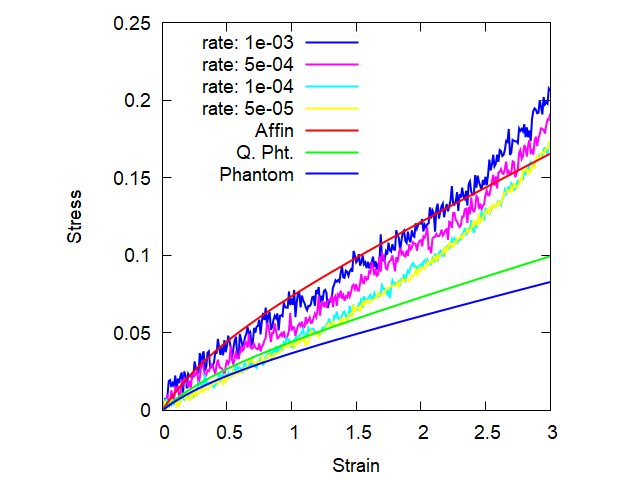
\includegraphics[width=\textwidth]{shear_random_4_N20.png}
%         \caption{Stress-Strain Curves for 4-chain NW at varied shear rate (1e-3 $\sim$ 5e-5 /$\tau$).}
%         \label{fig:deform}
%         \end{center}
%     \end{minipage}
%     \begin{minipage}{0.33\hsize}
%         \begin{center}
%         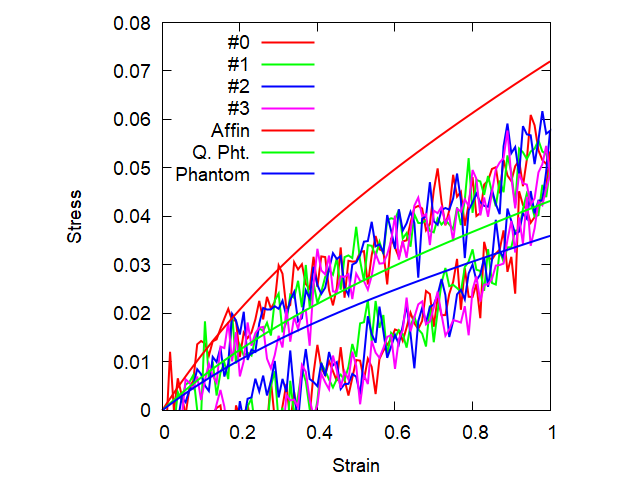
\includegraphics[width=\textwidth]{cyclic_shear_5e-4.png}
%         \caption{Hysteresis Curves for 4-chain NW by Cyclic Shear: shear rate 5e-4}
%         \label{fig:hyst}
%         \end{center}
%     \end{minipage}
%     \begin{minipage}{0.33\hsize}
%         \begin{center}
%         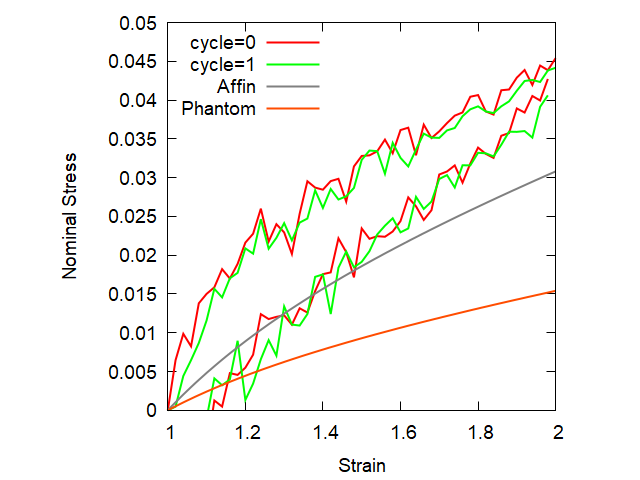
\includegraphics[width=\textwidth]{hyst_4Chain.png}
%         \caption{Strand Exchange Procedure}
%         \label{fig:exc}
%         \end{center}
%     \end{minipage}
% \end{figure}

\begin{figure}[hb]
    \begin{minipage}{0.5\hsize}
        \begin{center}
        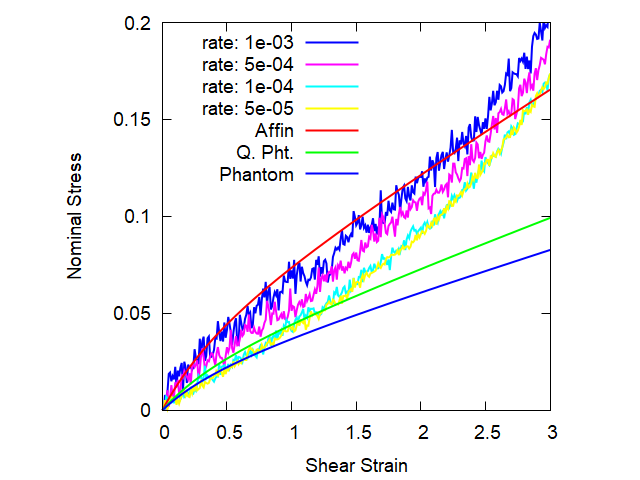
\includegraphics[width=.7\textwidth]{Shear_Random_4chain_N20.png}
        \caption{Stress-Strain Curves for 4-chain NW at varied shear rate (1e-2 $\sim$ 5e-5 $\lambda/\tau$)}
        \label{fig:deform}
        \end{center}
    \end{minipage}
    \begin{minipage}{0.5\hsize}
        \begin{center}
        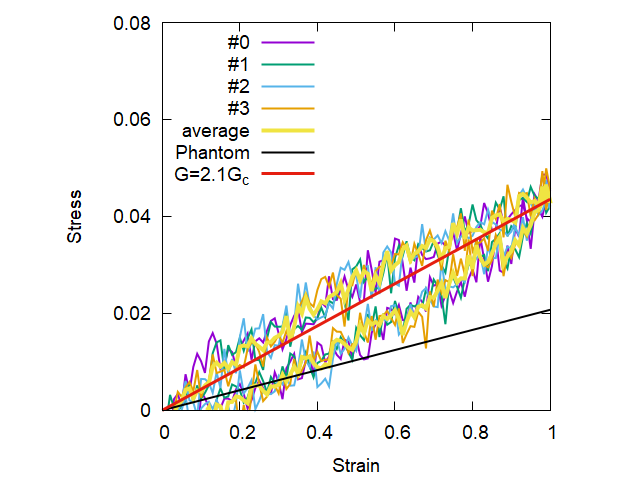
\includegraphics[width=.7\textwidth]{CyclicDeform_4chain_rate_2e-4.png}
        \caption{Hysteresis Curves for 4-chain NW by Cyclic Shear ($\lambda = 1$): shear rate 2e-4 $\lambda/\tau$}
        \label{fig:hyst}
        \end{center}
    \end{minipage}
    % \begin{minipage}{0.33\hsize}
    %     \begin{center}
    %     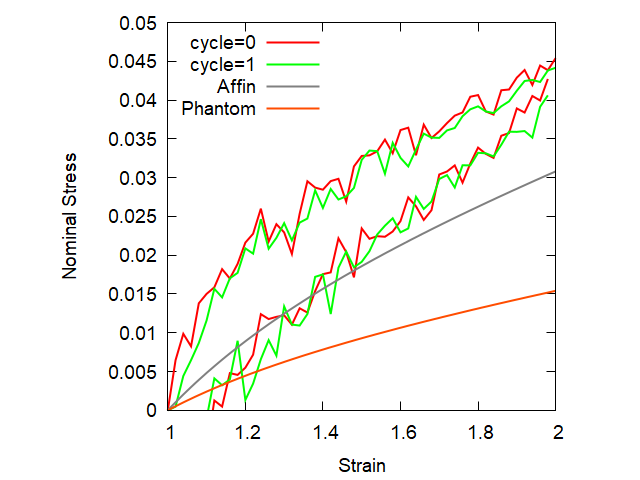
\includegraphics[width=\textwidth]{hyst_4Chain.png}
    %     \caption{Strand Exchange Procedure}
    %     \label{fig:exc}
    %     \end{center}
    % \end{minipage}
\end{figure}


\begin{thebibliography}{99}
    \bibitem{andrews} E. H. Andrews, Y. Fukahori Journal of Materials Science, 12, 1307 (1977)
    \bibitem{smith} T. L. Smith, R. A. Dickie Journal of Polymer Science Part A-2: Polymer Physics, 7, 635 (1969)
    \bibitem{flory} P. J. Flory Proceedings of the Royal Society of London. Series A, 351, 351 (1976)
    \bibitem{sasaki} H. Sasaki, 69th Rheology Symposium Preprint (2021)
\end{thebibliography}

\end{document}